\documentclass[12pt,a4paper]{article}

% Language setting
\usepackage[british]{babel}

% Set page size and margins
\usepackage[a4paper,top=2cm,bottom=2cm,left=2.5cm,right=2.5cm,marginparwidth=1.75cm]{geometry}

%----------- APA style references & citations (starting) ---
% Useful packages
%\usepackage[natbibapa]{apacite} % APA-style citations.

\usepackage[style=apa, backend=biber]{biblatex} % APA 7th edition style citations using bib latex
\addbibresource{refs.bib} % Your .bib file

% Formatting DOI in APA-7 style
%\renewcommand{\doiprefix}{https://doi.org/}

% Add additional APA 7th edition requirements
\DeclareLanguageMapping{british}{british-apa} % Set language mapping
\DeclareFieldFormat[article]{volume}{\apanum{#1}} % Format volume number

% Modify 'and' to '&' in the bibliography
\renewcommand*{\finalnamedelim}{%
  \ifnumgreater{\value{liststop}}{2}{\finalandcomma}{}%
  \addspace\&\space}
  
%----------- APA style references & citations (ending) ---


\usepackage{amsmath}
\usepackage{graphicx}
\usepackage[colorlinks=true, allcolors=blue]{hyperref}
\usepackage{hyperref}
%\usepackage{orcidlink}
\usepackage[title]{appendix}
\usepackage{mathrsfs}
\usepackage{amsfonts}
\usepackage{booktabs} % For \toprule, \midrule, \botrule
\usepackage{caption}  % For \caption
\usepackage{threeparttable} % For table footnotes
\usepackage{algorithm}
\usepackage{algorithmicx}
\usepackage{algpseudocode}
\usepackage{listings}
\usepackage{enumitem}
\usepackage{chngcntr}
\usepackage{booktabs}
\usepackage{lipsum}
\usepackage{subcaption}
\usepackage{authblk}
\usepackage[T1]{fontenc}    % Font encoding
\usepackage{csquotes}       % Include csquotes
\usepackage{diagbox}
\usepackage{comment}
\usepackage{siunitx}


% Customize line spacing
\usepackage{setspace}
\onehalfspacing % 1.5 line spacing

% Redefine section and subsection numbering format
\usepackage{titlesec}
\titleformat{\section} % Redefine section numbering format
  {\normalfont\Large\bfseries}{\thesection.}{1em}{}
  
%% Customize line numbering format to right-align line numbers
%\usepackage{lineno} % Add the lineno package
%\renewcommand\linenumberfont{\normalfont\scriptsize\sffamily\color{blue}}
%\rightlinenumbers % Right-align line numbers
%
%\linenumbers % Enable line numbering

% Define a new command for the fourth-level title.
\newcommand{\subsubsubsection}[1]{%
  \vspace{\baselineskip}% Add some space
  \noindent\textbf{#1\\}\quad% Adjust formatting as needed
}
% Change the position of the table caption above the table
\usepackage{float}   % for customizing caption position
\usepackage{caption} % for customizing caption format
\captionsetup[table]{position=top} % caption position for tables

%% Define the unnumbered list
%\makeatletter
%\newenvironment{unlist}{%
%  \begin{list}{}{%
%    \setlength{\labelwidth}{0pt}%
%    \setlength{\labelsep}{0pt}%
%    \setlength{\leftmargin}{2em}%
%    \setlength{\itemindent}{-2em}%
%    \setlength{\topsep}{\medskipamount}%
%    \setlength{\itemsep}{3pt}%
%  }%
%}{%
%  \end{list}%
%}
%\makeatother

% Suppress the warning about \@parboxrestore
\pdfsuppresswarningpagegroup=1

%-------------------------------------------
% Paper Head
%-------------------------------------------
\title{What makes for effective pandemic policy?}

\author{David Yuan, Nathan Cantafio}

\date{}  % Remove date

\begin{document}
\maketitle

\begin{abstract}
In light of the COVID-19 pandemic, understanding the impact of public health interventions on epidemic spread has become crucial for managing future outbreaks. A common framework for pandemic modelling is the SIR (Susceptible/Infected/Recovered) model which uses differential equations to model disease spread. There are many extensions of this model that add more groups (such as SIVQR -- Susceptible/Infected/Vaccinated/Quarantined/Recovered), and there are innumerable different policy interventions/characteristics of the disease one can consider in the model. This report aims to determine which policy measures are most important in managing disease spread.
\end{abstract} 

%-------------------------------------------
% Paper Body
%-------------------------------------------
\section{Introduction}\label{section1}

%You need to say enough to understand the problem and objectives and a
%quick guide to your approach. At the end of the introduction, give a brief outline of what
%the following sections will cover, e.g., ``The rest of the report is as follows. Details of the
%experimental design will be given in Section 2, . . .''
%Probably we will cite here

The question of interest is determining which policy levers are the most effective at managing disease spread during an outbreak. Some examples of policy levers are a quarantine policy for infected individuals, blanket social distancing measures, mask mandates, vaccine programs, etc. Inspired by the model presented in \cite{TURKYILMAZOGLU2022127429}, we will simulate the evolution of a pandemic under various scenarios. 

To measure how effective a particular strategy is, we would like to look at the resulting load on the healthcare system. This depends on how many people get sick, what kinds of people are getting sick (is it mostly elderly or healthy young people?), how long they are sick for. If at any point the load is too high for the healthcare system to handle, people will be left without treatment and potentially die. Thus we aim to keep the maximum load over the entire period as low as possible, i.e. we want to ``flatten the curve''.

In practice, we don't have a way of directly measuring the load. A good proxy however, is the total number of people who are sick. Which in our model includes those who are infectious and the infectious people who have been put in quarantine.

The remainder of this report is organized as follows: Section~\ref{section2} outlines the experimental design, highlighting the rationale behind factor selection and level choices. Section~\ref{section3} presents the results of simulations and statistical analyses. Section~\ref{section4} delves into the implications of these results, offering insights and  recommendations for policymakers. The Appendix includes more in depth discussion of the model and the simulation setup, as well as all the relevant tables and figures.

\section{The experimental design}\label{section2}

In the \verb`MATLAB` code there are eight parameters of interest that we can tune. They are in no particular order:  \verb`prob_spread`, \verb`recovery_rate`, \verb`vac_eff`, \verb`prob_sympt`,  \verb`isolation`,  \verb`vac_rate`, \verb`quar_dur`, \verb`num_daily`.

These represent (respectively) the probability that an unvaccinated individual will catch the disease from a single interaction with an infectious individual, the average rate of recovery for an infected individual in days, the proportional effectiveness of the vaccine (for example 0.1 means that vaccinated individuals are 10\% as likely to get infected compared to if they were unvaccinated), the probability that an infected individual shows symptoms, the social isolation policy in place (i.e. at the extreme ends: a social isolation policy of 0 corresponds to a policy that leads to no reduction in the number of daily interactions, and a social isolation policy of 1 corresponds to a policy that leads to a 90\% reduction in the number of daily interactions), the rate at which the susceptible population is vaccinated in days, the duration that symptomatic individuals are quarantined in days, the average number of daily interactions that have the potential to spread the disease that an individual has per day. 

The first of four of these parameters were randomized in simulation for each observation. This choice was made to reduce the number of effective runs, and because these parameters are traits of the particular disease and would be hard (or potentially impossible) to measure in the real world. More detail is given in Appendix~\ref{appendixA} and Table~\ref{tab:randomization_summary}. The last four of these parameters were considered as factors and their levels were thus pre-designed and recorded. 

The design is a full $3^4$ factorial. For a summary of the experimental factors, see Table~\ref{tab:factor_summary}. These levels were chosen to be realistic so that they would provide useful information and to cover a wide range of possibilities without increasing the size of the experiment excessively. The levels of \verb`soc.iso` were chosen to capture the three main types of policy: no policy, somewhat lax ``social distancing'', and harsher lockdowns where nobody interacts with anybody except for what is absolutely necessary. The levels of \verb`vac.rate` were chosen based on data in \cite{WHO} where the highest rates range between about 1--2\% of the population vaccinated per day and the lowest level 0\% serves as baseline with no vaccination. The levels of \verb`quar.dur` were chosen based on the 7 and 14 day quarantine periods having been common recommendations during the COVID-19 pandemic, again with 0 days (no quarantine) serving as a baseline. The levels of \verb`num.daily` were chosen to block for variation in population density between different regions. This is a hard number to estimate, but based on data from \cite{contacts} we think that between 15 to 45 interactions per day which would correspond to moderately suburban areas and highly dense city centres respectively is reasonable.

The response of interest is \verb`load` which is defined as the maximum proportion of sick (infectious or quarantined) individuals over 90 days. For a full description see Appendix~\ref{appendixB}.

 The model equation is:
\vspace*{-3mm}
\begin{align*}
	Y_{ijk\ell}=\mu+\alpha_i+\nu_j+\kappa_k+\eta_\ell+(\alpha\nu)_{ij}+(\alpha\kappa)_{ik}+(\alpha\eta)_{i\ell}+(\nu\kappa)_{jk}+(\nu\eta)_{j\ell} + (\kappa\eta)_{k\ell}\\
	+(\alpha\nu\kappa)_{ijk}+(\alpha\nu\eta)_{ij\ell}+(\alpha\kappa\eta)_{ik\ell} + (\nu\kappa\eta)_{jk\ell} + (\alpha\nu\kappa\eta)_{ijk\ell}+E_{ijk\ell}
\end{align*}
\vspace*{-10mm}

where $i,j,k,\ell\in\{1,2,3\}$ and a full description of the terms is contained in Table~\ref{tab:model_equation}

\section{Analysis}\label{section3}

We begin by verifying the model assumptions. Looking at the Box-Cox plot in Figure~\ref{fig:boxcox} we see that no transformation of the data is reasonable. Furthermore the  residual plot [Figure~\ref{fig:residuals}], and quantile plot [Figure~\ref{fig:qqplot}] show that assumptions about the error and form of our model are reasonable.

Referring to Table~\ref{tab:anova} none of the higher order effects are statistically significant, so with that in mind the remainder of this report will only consider main effects. Of these primary factors, \verb`soc.iso`, \verb`quar.dur`, and \verb`num.daily` all have statistically significant effects on \verb`load` at the $0.1\%$ level. While \verb`rate.vac` is only significant at the $10\%$ level.

From the Figure~\ref{fig:boxplot_soc.iso} we see there is a large reduction in \verb`load` when changing \verb`soc.iso` from levels 0 or 0.5 to level 1. This indicates that when it comes to social distancing policies, half measures are not nearly as effective in terms of minimizing \verb`load`. This is supported by the contrasts provided in Table~\ref{tab:contrasts}

box plots (contrasts?)

estimated effects/slopes

recommended levels and estimated load at rec levels

- estimated effects, box plots, recommended levels for each level of num.daily, estimated load at those recommended levels
	
%Try to be specific about your findings, and present numerical
%estimated effects, recommended levels, the estimated response at the recommended levels,
%etc. ``The high level of temperature was better at the 5\% significance level'' does not
%summarize well: the reader would have to make some more calculations to assess whether
%the result is practically significant. Instead, ``We are 95\% confident that the effect of
%changing temperature from 15 to 25°C is an increase in mean (a response variable) of (a
%confidence interval)'' tells the reader immediately whether there is a result of concern.
%
%If interaction effects are reported you should be careful to interpret them. Numerical
%estimates of interaction effects are not easy to understand. Rather, refer to a table of
%averages or an interaction plot. Talk about how the estimated effect of one factor depends
%on the level of another.
%
%Do not give excessive digits for estimates, etc. Two significant digits are usually sufficient
%for a standard error. Give the corresponding estimate to the same accuracy, e.g., 14.37 kg
%with standard error 0.54 kg, 14.4 kg with standard error 5.4 kg, or 14 kg with standard
%error 54 kg. Always give units of measurement for estimates and standard errors.
%
%If a transformation has been applied you will often want to convert predictions on the
%transformed scale back to the original scale.

\section{Conclusions}\label{section4}

Summarize results.



Vaccine rates were seen to be much less influential compared to our expectations. It's possible that vaccines are more useful as a tool for preventing future outbreaks, more so than managing present ones. With that in mind, a future experiment could consider varying initial conditions with different proportions of the population initially vaccinated.







%-------------------------------------------
% Appendix
%-------------------------------------------
% Activate the appendix in the doc
% from here on sections are numerated with capital letters 
%\appendix

\begin{appendices}

\newpage
\section*{Appendix}
%--- Section ---%
\section{Discussion of simulation}\label{appendixA}

The model considers five distinct groups: $S$, $I$, $V$, $Q$, and $R$; which are the number of susceptible, infected, vaccinated, quarantined and recovered individuals respectively. If $N$ is the total population, we can define $s=S/N$, $i=I/N$, $v=V/N$, $q=Q/N$, $r=R/N$ and work with these population proportions. The system of differential equations is
\begin{equation}
	\begin{cases}
	ds/dt = -\beta_0si-\nu s\\
	di/dt = \beta_0si + \beta_1 vi - \mathbb{I}_QP_\text{sympt}i+(1-\gamma_Q)\kappa q - \gamma i\\
	dv/dt = \nu s - \beta_1	vi\\
	dq/dt = \mathbb{I}_QP_\text{sympt}i - \kappa q\\
	dr/dt = \gamma i +\gamma_Q\kappa q
	\end{cases}
\end{equation}
where 
\vspace*{-3mm}
\begin{itemize}
	\item $\beta_0$ and $\beta_1$ are the transmission rate ($\text{\# daily interactions}\times\mathbb{P}[\text{spread per interaction}]$) for unvaccinated and vaccinated individuals respectively
	\vspace*{-3mm}
	\item $\nu$ is the vaccination rate of susceptible individuals
	\vspace*{-3mm}
	\item $\mathbb{I}_Q$ is an indicator variable equalling $1$ if there is a quarantine policy and $0$ if there is no quarantine policy
	\vspace*{-3mm}
	\item $P_\text{sympt}$ is the probability that an infected individual is symptomatic
	\vspace*{-3mm}
	\item $\gamma$ and $\gamma_Q$ are the average rates [$1/(\text{average recovery duration})$] of recovery for infected individuals and individuals who just came out of quarantine respectively
	\vspace*{-3mm}
	\item $\kappa$ is the average rate [$1/(\text{average quarantine duration})$] at which we take people out of quarantine
\end{itemize}
The \verb`MATLAB` code uses Euler's method with time steps of size \verb`k = 0.001` to simulate the dynamics of these groups up to \verb`Tf = 90` days from an initial condition of $1\%$ infected and everyone else susceptible. Parameters mentioned to be randomized in Section~\ref{section2} were done so using the built in functions \verb`randn()`. The range of possible values are shown in Table~\ref{tab:randomization_summary}. The response was measured as \verb`load = max(i + q)`.

\section{Description of data}\label{appendixB}
Explain all variables...

\section{Tables and figures}\label{appendixC}

% table 1
\begin{table}[H]
    \centering
    \begin{tabular}{l l l}\hline
         Factor &  Levels & Symbol \\ \hline\hline
         Isolation & Low (0), Medium (0.5), High (1) & \verb`soc.iso` \\ \hline
         Vaccination rate & 0 \si{ppd}, 1 \si{ppd}, 2 \si{ppd} & \verb`vac.rate` \\ \hline
         Quarantine duration & 0 days, 7 days, 14 days & \verb`quar.dur`\\ \hline
         Average number of daily interactions & 15 \si{ipd}, 30 \si{ipd}, 45 \si{ipd} & \verb`num.daily` \\ \hline \\
    \end{tabular}
    \caption{\si{ppd} is ``percent population vaccinated per day'' and \si{ipd} is ``average number of daily interactions per day''}
    \label{tab:factor_summary}
\end{table}

\begin{table}[H]
    \centering
    \begin{tabular}{l l l}\hline
         Parameter &  Range & Variable name \\ \hline\hline
         Probability of spread per interaction & $[0.05,0.15]$ & \verb`prob_spread` \\ \hline
         Recovery rate & $[7,21]$ days & \verb`recovery_rate` \\ \hline
         Vaccine effectiveness & $[40\%,60\%]$ & \verb`vac_eff`\\ \hline
         Proportion sympomatic  & $[0, 0.6]$ & \verb`prob_sympt` \\ \hline \\
    \end{tabular}
    \caption{The above parameters were uniformly generated from the corresponding range}
    \label{tab:randomization_summary}
\end{table}

\begin{table}[H]
	\centering
	\begin{tabular}{l l}\hline
	Term & Description \\ \hline \hline
	$\mu$ & an effect common to all observations \\ \hline
	$\alpha_i$ & the effect on \verb`load` of \verb`soc.iso` at level $i$ \\ \hline
 	$\nu_j$ & the effect on \verb`load` of \verb`vac.rate` at level $j$ \\ \hline
	$\kappa_k$ & the effect on \verb`load` of \verb`quar.dur` at level $k$ \\ \hline
	$\eta_\ell$ & the effect on \verb`load` of \verb`num.daily` at level $\ell$ \\ \hline
	$(\alpha\nu)_{ij}$ & the ``interaction effect'' on \verb`load` of \verb`soc.iso` and \verb`vac.rate` \\ \hline
	other interactions terms & similar \\ \hline
	$E_{ijk\ell}$ & the residual error at levels $i,j,k,\ell$; distributed as $\mathcal{N}(0,\sigma^2)$ \\ \hline
	$Y_{ijk\ell}$ & the recorded value of \verb`load` at level $i,j,k,\ell$ \\ \hline \\
	\end{tabular}
	\caption{A description of terms in the model equation}
	\label{tab:model_equation}
\end{table}

% FIGURES
\begin{figure}[H]
	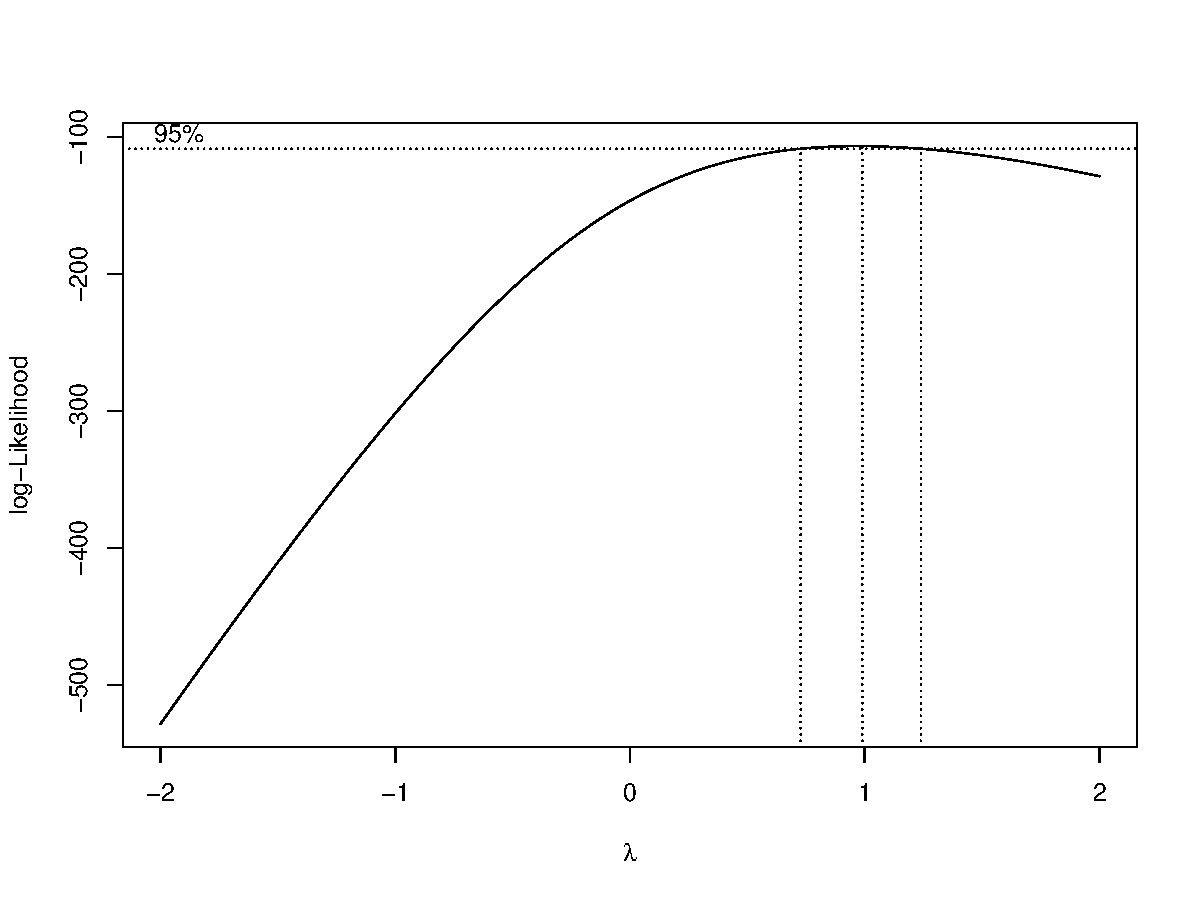
\includegraphics[width=\linewidth]{boxcox.pdf}
	\caption{Boxcox plot}	 % make better captions
	\label{fig:boxcox}
\end{figure}

\begin{figure}[H]
	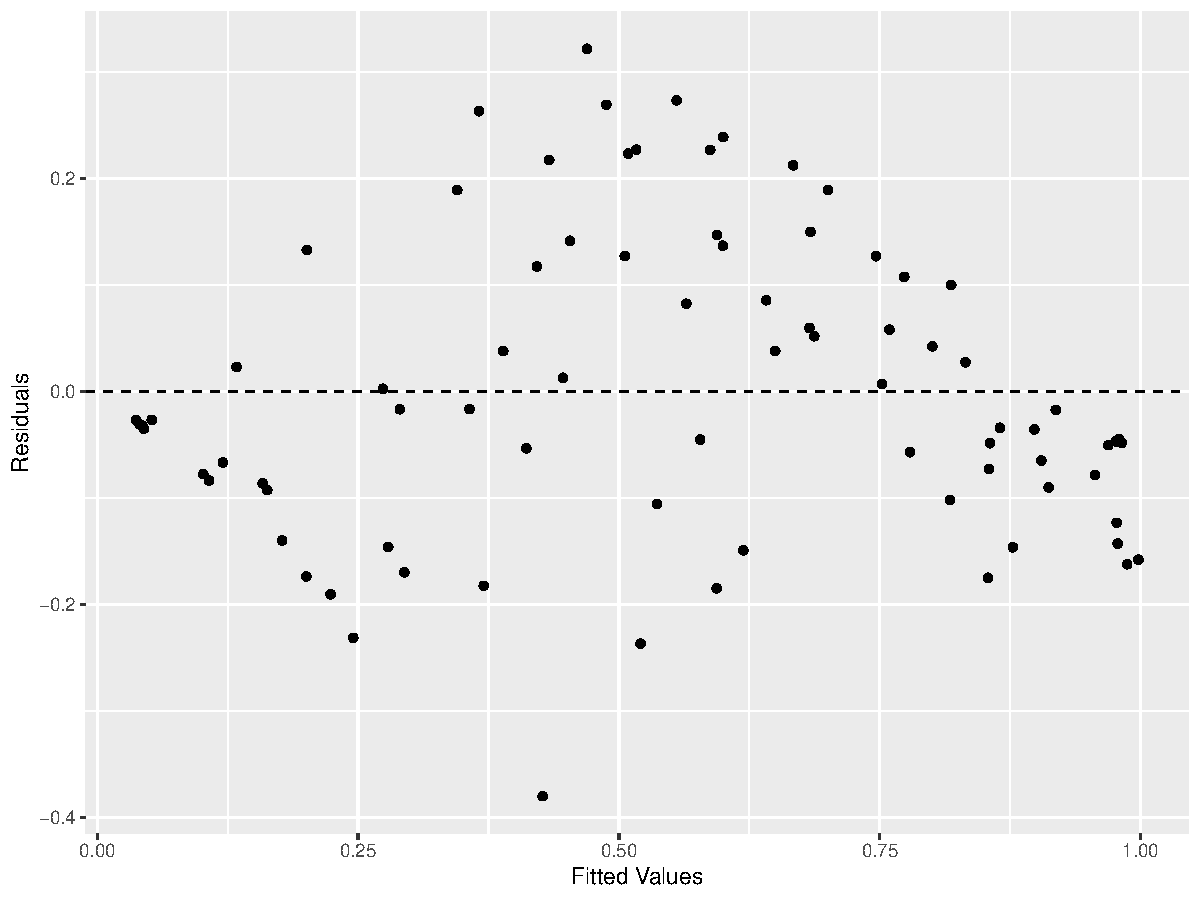
\includegraphics[width=\linewidth]{residuals.pdf}
	\caption{Residuals}	 % make better captions
	\label{fig:residuals}
\end{figure}

\begin{figure}[H]
	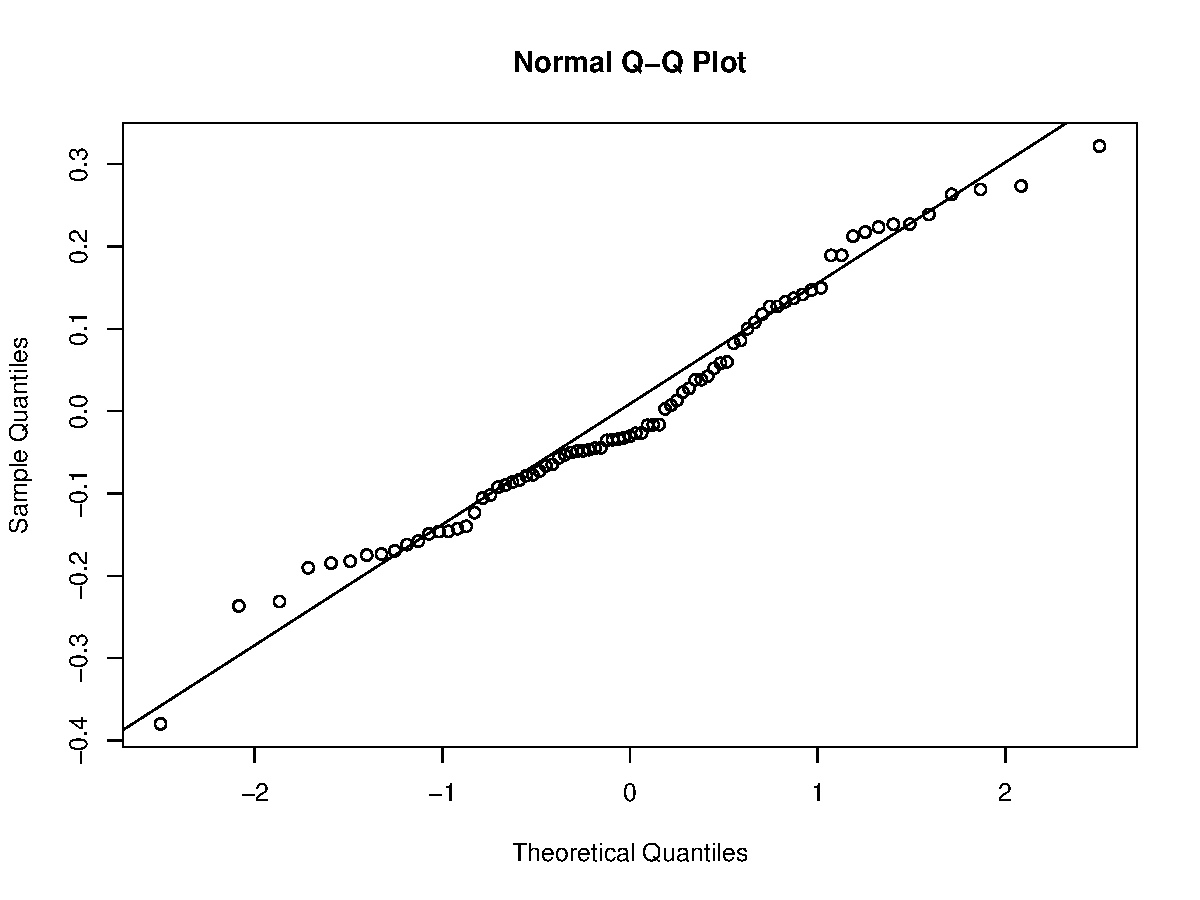
\includegraphics[width=\linewidth]{qqplot.pdf}
	\caption{Quantile plot}	 % make better captions
	\label{fig:qqplot}
\end{figure}







\end{appendices}

%-------------------------------------------
% References
%-------------------------------------------

% Print bibliography
\printbibliography




\end{document}